\documentclass[DaoFP]{subfiles}
\begin{document}
    \setcounter{chapter}{12}

    \chapter{Coalgebras(余代数)}

    Coalgebras(余代数)就是在对偶范畴中的代数(algebras)。到此为止,本章结束!

    不过,也许事情没有那么简单……正如我们之前所看到的,我们工作的范畴并不具有关于对偶性的对称性。特别是,如果我们比较终对象(terminal objects)和初对象(initial objects),它们的性质并不对称。我们的初对象没有入射箭头,而终对象除了拥有唯一的入射箭头外,还有许多出射箭头。

    由于初代数(initial algebras)是从初对象构造出来的,因此我们可能预期终余代数(terminal coalgebras)——作为它们的对偶,因此由终对象生成——不仅仅是它们的镜像,还会有一些有趣的变化。

    我们已经看到代数的主要应用是在处理递归数据结构时:在对它们进行折叠(folding)。与此对应,余代数的主要应用是在生成或展开(unfolding)递归的、类似树的数据结构。展开是通过一种称为anamorphism(异态射)的方式来完成的。

    我们使用catamorphisms(猫态射)来修剪树,而使用anamorphisms(异态射)来生成它们。

    我们无法凭空生成信息,所以一般来说,无论是catamorphism还是anamorphism,都会减少输入中包含的信息量。

    例如,当你对整数列表求和后,就无法恢复原始的列表了。

    同样地,如果你使用anamorphism生成递归数据结构,种子(seed)必须包含最终在树中呈现的所有信息。你没有获得新信息,但优势在于你拥有的信息现在以一种更方便进一步处理的形式存储了起来。

    \section{Coalgebras from Endofunctors(由自函子生成的余代数)}

    一个endofunctor(自函子)$F$的coalgebra(余代数)是一个包含载体(carrier)$a$和结构映射(structure map)的对:一个从$a \to F a$的箭头。

    在Haskell中,我们定义:
    \begin{haskell}
        type Coalgebra f a = a -> f a
    \end{haskell}
    我们通常将载体视为生成数据结构的种子类型,无论是列表还是树。

    例如,这里有一个可以用来创建二叉树的函子,整数存储在节点中:
    \begin{haskell}
        data TreeF x = LeafF | NodeF Int x x
        deriving (Show, Functor)
    \end{haskell}
    我们甚至不需要为它定义\hask{Functor}的实例——\hask{deriving}子句告诉编译器为我们生成规范的实例(以及允许将其转换为\hask{String}的\hask{Show}实例,如果我们想显示它的话)。

    一个coalgebra(余代数)是一个函数,它接受载体类型的种子并生成一个充满新种子的函子。这些新种子然后可以用于递归地生成子树。

    这里是一个为函子\hask{TreeF}定义的coalgebra(余代数),它将整数列表作为种子:
    \begin{haskell}
        split :: Coalgebra TreeF [Int]
        split [] = LeafF
        split (n : ns) = NodeF n left right
        where
        (left, right) = partition (<= n) ns
    \end{haskell}
    如果种子为空,它会生成一片叶子;否则它会创建一个新节点。这个节点存储列表的头部,并用两个新种子填充节点。库函数\hask{partition}使用用户定义的谓词分割列表,这里是\hask{(<= n)},小于或等于\hask{n}。结果是一个满足谓词的列表对,和一个不满足的列表对。

    你可以确信,递归地应用这个coalgebra(余代数)会创建一个二叉排序树。我们稍后将使用这个coalgebra实现一个排序。

    \section{Category of Coalgebras(余代数的范畴)}

    通过类似代数态射(algebra morphisms)的方式,我们可以定义余代数态射(coalgebra morphisms)为满足交换条件的载体之间的箭头。

    给定两个余代数$(a, \alpha)$和$(b, \beta)$,如果箭头$f \colon a \to b$使得下图交换,那么它就是一个余代数态射:
    \[
        \begin{tikzcd}
            a
            \arrow[r, "f"]
            \arrow[d, "\alpha"]
            & b
            \arrow[d, "\beta"]
            \\
            F  a
            \arrow[r, "F f"]
            & F b
        \end{tikzcd}
    \]

    其含义是,无论我们是先映射载体,然后应用余代数$\beta$,还是先应用余代数$\alpha$,然后对其内容应用通过函子提升的箭头$F f$,结果都是相同的。

    余代数态射可以组合,且恒等箭头自动是余代数态射。可以很容易地看出,余代数和代数一样,也形成一个范畴。

    然而,这次我们感兴趣的是这个范畴中的终对象——\emph{终余代数}。如果终余代数$(t, \tau)$存在,它就满足Lambek引理(Lambek's lemma)的对偶。

    \begin{exercise}{Lambek's lemma:}
        证明终余代数$(t, \tau)$的结构映射$\tau$是同构的。提示:证明过程与初代数的证明相对偶。
    \end{exercise}

    作为Lambek引理的结果,终代数的载体是该函子的一个不动点(fixed point)。
    \[ F t \cong t \]
    $\tau$和$\tau^{-1}$作为这种同构的证据。

    这也意味着$(t, \tau^{-1})$是一个代数;就像$(i, \iota^{-1})$是一个余代数一样,假设$(i, \iota)$是初代数。

    我们之前已经看到,初代数的载体是一个不动点。原则上,可能有许多相同自函子的不同不动点。初代数是最小的不动点,而终余代数是最大的。

    自函子$F$的最大不动点记为$\nu F$,因此我们有:
    \[ t = \nu F \]

    我们还可以看到,必然存在一个从初代数到终余代数的唯一代数态射(catamorphism)。这是因为终余代数也是一个代数。

    同样,必然存在一个从初代数(它也是一个余代数)到终余代数的唯一余代数态射。事实上,可以证明,在这两种情况下,它是同一个基础态射$\rho \colon \mu F \to \nu F$。

    在集合范畴中,初代数的载体集合是终余代数的载体集合的子集,函数$\rho$将前者嵌入后者。
    \[
        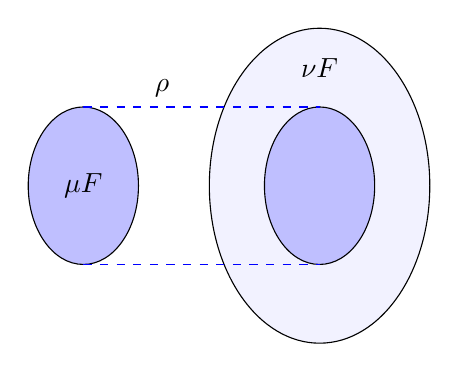
\begin{tikzpicture}
            \draw (-1,0)[fill=blue!25!white] ellipse (0.7 and 1);
            \draw (2,0)[fill=blue!5!white] ellipse (1.4 and 2);
            \draw (2,0)[fill=blue!25!white] ellipse (0.7 and 1);
            \node[above] at (0, 1) {$\rho$};
            \draw[dashed, blue] (-1, 1) -- (2, 1);
            \draw[dashed, blue] (-1, -1) -- (2, -1);
            \node at (-1, 0) { $\mu F$ };
            \node at (2, 1.5) { $\nu F$ };
        \end{tikzpicture}
    \]

    我们稍后会看到,在Haskell中,由于惰性求值的原因,情况更为微妙。但至少对于那些具有叶节点成分的函子——即它们在初对象上的作用是非平凡的——Haskell的固定点类型可作为初代数和终余代数的载体。
    \begin{haskell}
        data Fix f where
        In :: f (Fix f) -> Fix f
    \end{haskell}

    \begin{exercise}
        证明在$\mathbf{Set}$中的恒等函子中,每个对象都是一个不动点,空集是最小的不动点,而单集合是最大的。提示:最小的不动点必须有箭头指向所有其他不动点,而最大的不动点必须有箭头从所有其他不动点指向它。
    \end{exercise}

    \begin{exercise}
        证明空集是$\mathbf{Set}$中恒等函子的初代数的载体。对偶地,证明单集合是这个函子的终余代数。提示:证明这些唯一箭头确实是(余)代数态射。
    \end{exercise}

    \section{Anamorphisms(异态射)}

    终余代数$(t, \tau)$通过其泛性质(universal property)定义:从任何余代数$(a, \alpha)$到$(t, \tau)$的唯一余代数态射$h$被称为\emph{异态射}(anamorphism)。作为一个余代数态射,它使下图交换:
    \[
        \begin{tikzcd}
            a
            \arrow[r, dashed, "h"]
            \arrow[d, "\alpha"]
            & t
            \arrow[d, "\tau"]
            \\
            F a
            \arrow[r,  "F h"]
            & F t
        \end{tikzcd}
    \]

    就像代数一样,我们可以使用Lambek引理来“求解”$h$:
    \[ h = \tau^{-1} \circ F h \circ \alpha \]
    这种解法被称为anamorphism(异态射),有时用“镜片括号”(lens brackets)$\llens \alpha \rlens$表示。

    由于终余代数(与初代数一样)是函子的一个不动点,上述递归公式可以直接翻译为Haskell代码:
    \begin{haskell}
        ana :: Functor f => Coalgebra f a -> a -> Fix f
        ana coa = In . fmap (ana coa) . coa
    \end{haskell}
    这里是该公式的解释:给定类型为\hask{a}的种子,我们首先对其应用余代数\hask{coa}。这会给我们一个充满种子的函子。我们通过递归地应用异态射使用\hask{fmap}扩展这些种子。然后我们应用构造器\hask{In}得到最终结果。

    例如,我们可以将异态射应用于我们之前定义的\hask{split}余代数:\hask{ana split}接受一个整数列表并创建一个排序树。

    然后我们可以使用一个catamorphism来将这个树折叠成一个排序列表。我们定义以下代数:
    \begin{haskell}
        toList :: Algebra TreeF [Int]
        toList LeafF = []
        toList (NodeF n ns ms) = ns ++ [n] ++ ms
    \end{haskell}
    它将左侧列表与单元素枢轴和右侧列表连接起来。要对列表进行排序,我们将anamorphism与catamorphism结合起来:
    \begin{haskell}
        qsort = cata toList . ana split
    \end{haskell}
    这给了我们一个(非常低效的)快速排序实现。我们将在下一节中进一步讨论这个问题。

    \subsection{Infinite data structures(无限数据结构)}

    在研究代数时,我们依赖于具有叶节点成分的数据结构——即当自函子作用于初对象时,会产生与初对象不同的结果。构造递归数据结构时,我们必须从某个地方开始,这意味着首先构造叶子。

    对于余代数,我们可以自由地放弃这个要求。我们不再需要“手工”构造递归数据结构——我们有anamorphisms来为我们做这件事。一个没有叶子的自函子是完全可以接受的:它的余代数将生成无限的数据结构。

    在Haskell中,由于其惰性求值,无限数据结构是可表示的。只有显式要求的那些部分才会被计算,剩余部分则保持在挂起状态。

    要在严格语言中实现无限数据结构,必须使用函数来表示值——这在Haskell中是幕后完成的(这些函数称为“thunks”)。

    让我们看一个简单的例子:一个无限的值流。要生成它,我们首先定义一个看起来很像我们用来生成列表的函子,除了它缺少叶节点成分(空列表构造器)。你可能会将其识别为乘积函子,第一成分固定为流的有效负载:
    \begin{haskell}
        data StreamF a x = StreamF a x
        deriving Functor
    \end{haskell}
    一个无限流是这个函子的固定点。
    \begin{haskell}
        type Stream a = Fix (StreamF a)
    \end{haskell}
    这是一个简单的余代数,它使用单个整数\hask{n}作为种子:
    \begin{haskell}
        step :: Coalgebra (StreamF Int) Int
        step n = StreamF n (n+1)
    \end{haskell}
    它将当前种子存储为有效负载,并用\hask{n + 1}为下一个流生成种子。

    这个余代数的异态射,当种子为零时,生成所有自然数的流。
    \begin{haskell}
        allNats :: Stream Int
        allNats = ana step 0
    \end{haskell}
    在非惰性语言中,这个异态射将永远运行,但在Haskell中它是瞬时的。只有当我们想要检索一些数据时,才会逐步支付成本,例如,使用这些访问器:
    \begin{haskell}
        head :: Stream a -> a
        head (In (StreamF a _)) = a

        tail :: Stream a -> Stream a
        tail (In (StreamF _ s)) = s
    \end{haskell}


    \section{Hylomorphisms(合态射)}

    anamorphism的输出类型是函子的固定点,这与catamorphism的输入类型相同。在Haskell中,它们都由相同的数据类型\hask{Fix f}描述。因此我们可以将它们组合在一起,就像我们在实现快速排序时所做的那样。事实上,我们可以将余代数与代数结合在一个递归函数中,称为\emph{合态射}(hylomorphism):
    \begin{haskell}
        hylo :: Functor f => Algebra f b -> Coalgebra f a -> a -> b
        hylo alg coa = alg . fmap (hylo alg coa) . coa
    \end{haskell}
    我们可以将快速排序重写为一个hylomorphism:
    \begin{haskell}
        qsort = hylo toList split
    \end{haskell}

    注意,在hylomorphism的定义中没有固定点的踪迹。从概念上讲,余代数用于从种子生成(展开)递归数据结构,而代数用于将其折叠成\hask{b}类型的值。但由于Haskell的惰性求值,中间数据结构不必在内存中完全实体化。这在处理非常大的中间树时尤其重要。只有当前正在遍历的分支被评估,一旦它们被处理完毕,它们就会被传递给垃圾收集器。

    在Haskell中,hylomorphisms是递归回溯算法的一个方便替代,而递归回溯算法在命令式语言中非常难以正确实现。我们利用了一个事实,即设计数据结构比跟踪复杂的控制流和记住递归算法中的位置要容易得多。

    通过这种方式,数据结构可以用于可视化复杂的控制流。

    \subsection{The impedance mismatch(阻抗不匹配)}

    我们已经看到,在集合范畴中,初代数不一定与终余代数重合。例如,恒等函子具有空集作为其初代数的载体,而具有单集合作为其终余代数的载体。

    我们还有其他没有叶节点成分的函子,例如流函子。这样的函子的初代数也是空集。

    在$\mathbf{Set}$中,初代数是终余代数的子集,合态射只能定义在这个子集中。这意味着我们只能在特定的余代数的anamorphism落入这个子集时使用合态射。在这种情况下,由于初代数在终余代数中的嵌入是单射的,我们可以找到初代数中的相应元素并对其应用catamorphism。

    然而,在Haskell中,我们有一种类型\hask{Fix f},它同时结合了初代数和终余代数。这就是将Haskell类型简单解释为值的集合的局限性。

    让我们考虑这个简单的流代数:
    \begin{haskell}
        add :: Algebra (StreamF Int) Int
        add (StreamF n sum) = n + sum
    \end{haskell}
    没有什么能阻止我们使用合态射来计算所有自然数的和:
    \begin{haskell}
        sumAllNats :: Int
        sumAllNats = hylo add step 1
    \end{haskell}
    这是一个完全有效的Haskell程序,通过了类型检查器。那么,当我们运行它时,它会生成什么值呢?(提示:它不是$-1/12$。)答案是:我们不知道,因为这个程序永远不会终止。它进入了无限递归,并最终耗尽了计算机的资源。

    这是现实计算中函数之间的集合模型无法模拟的一个方面。一些计算机函数可能永远不会终止。

    递归函数在形式上通过“域理论”(domain theory)描述为部分定义函数的极限。如果函数未对特定的参数值定义,则该函数被认为返回一个底值$\bot$。如果我们将底值作为每种类型的特殊元素(这些类型称为\emph{提升类型}(lifted types)),我们可以说我们的函数\hask{sumAllNats}返回了一个\hask{Int}类型的底值。一般来说,针对无限类型的catamorphisms不会终止,因此我们可以将它们视为返回底值。

    然而,应该注意的是,底值的引入复杂了Haskell的范畴解释。特别是,许多依赖于唯一性的映射的泛化构造不再如预期那样工作。

    “底线”是,Haskell代码应该被视为范畴概念的一个说明,而不是严格证明的来源。

    \section{Terminal Coalgebra from Universality(从泛性质推导的终余代数)}

    异态射的定义可以看作是终余代数的泛性质的一种表达。这里是它的定义,带有显式的泛量化:
    \begin{haskell}
        ana :: Functor f => forall a. Coalgebra f a -> (a -> Fix f)
        ana coa = In . fmap (ana coa) . coa
    \end{haskell}
    它告诉我们,给定任何余代数,从其载体到终余代数的载体\hask{Fix f}都有一个映射。我们知道,通过Lambek引理,这个映射实际上是一个余代数态射。

    让我们将这个定义的参数展开:
    \begin{haskell}
        ana :: Functor f => forall a. (a -> f a, a) -> Fix f
        ana (coa, x) = In (fmap (curry ana coa) (coa x))
    \end{haskell}
    我们可以将此公式用作终余代数载体的替代定义。我们可以将\hask{Fix f}替换为我们正在定义的类型——让我们称之为\hask{Nu f}。类型签名:
    \begin{haskell}
        forall a. (a -> f a, a) -> Nu f
    \end{haskell}
    告诉我们,我们可以从一个对\hask{(a -> f a, a)}构造出\hask{Nu f}的一个元素。它看起来就像一个数据构造器,除了它在\hask{a}上是多态的。

    具有多态构造器的数据类型称为\emph{存在类型}(existential types)。在伪代码中(非实际的Haskell),我们可以定义\hask{Nu f}为:
    \begin{haskell}
        data Nu f = Nu (exists a. (Coalgebra f a, a))
    \end{haskell}
    将其与最小不动点代数的定义进行比较:
    \begin{haskell}
        data Mu f = Mu (forall a. Algebra f a -> a)
    \end{haskell}

    要构造一个存在类型的元素,我们可以选择最方便的类型——我们有构造器所需的数据的类型。

    例如,我们可以通过选择\hask{Int}作为方便类型,并提供以下对来构造类型\hask{Nu (StreamF Int)}的一个项:
    \begin{haskell}
        nuArgs :: (Int -> StreamF Int Int, Int)
        nuArgs =  (\n -> StreamF n (n+1) , 0)
    \end{haskell}

    存在类型的客户端无法知道其构造时所使用的类型是什么。他们只知道这种类型“存在”——因此得名。如果他们想要使用一个存在类型,他们必须以一种不敏感于构造时所做选择的方式使用它。实际上,这意味着存在类型必须同时携带生成器和消费者。

    在我们的示例中确实如此:生成器只是\hask{a}类型的值,而消费者是\hask{a -> f a}函数。

    天真地说,客户端对这一对能做的唯一操作是在不知道\hask{a}是什么类型的情况下,将函数应用于值。但如果\hask{f}是一个函子,他们可以做得更多。他们可以通过将提升的函数应用于\hask{f a}的内容来重复这一过程,依此类推。他们最终得到无限流中包含的所有信息。

    在Haskell中有几种定义存在数据类型的方法。我们可以直接将异态射的未展开版本用作数据构造器:
    \begin{haskell}
        data Nu f where
        Nu :: forall a f. (a -> f a, a) -> Nu f
    \end{haskell}
    注意,在Haskell中,如果我们显式地量化了一个类型,所有其他类型变量也必须量化:这里是类型构造器\hask{f}(然而,\hask{Nu f}在\hask{f}上不是存在的,因为它是一个显式参数)。

    我们还可以完全省略量化:
    \begin{haskell}
        data Nu f where
        Nu :: (a -> f a, a) -> Nu f
    \end{haskell}
    这是因为不属于类型构造器的参数的类型变量自动被视为存在类型。

    我们还可以使用更传统的形式:
    \begin{haskell}
        data Nu f = forall a. Nu (a -> f a, a)
    \end{haskell}
    (这个版本需要对\hask{a}进行量化。)

    在撰写本文时,有一个提案引入关键字\hask{exists}到Haskell中,这样可以使以下定义生效:
    \begin{haskell}
        data Nu f = Nu (exists a. (a -> f a, a))
    \end{haskell}
    (稍后我们将看到,存在数据类型对应于范畴论中的余端(coends)。)

    \hask{Nu f}的构造器实际上就是异态射的未展开版本:
    \begin{haskell}
        anaNu :: Coalgebra f a -> a -> Nu f
        anaNu coa a = Nu (coa, a)
    \end{haskell}

    如果我们得到了一个\hask{Nu (StreamF a)}形式的流,我们可以使用访问函数提取其元素。这个函数提取第一个元素:
    \begin{haskell}
        head :: Nu (StreamF a) -> a
        head (Nu (unf, s)) =
        let (StreamF a _) = unf s
        in a
    \end{haskell}
    这个函数推进流:
    \begin{haskell}
        tail :: Nu (StreamF a) -> Nu (StreamF a)
        tail (Nu (unf, s)) =
        let (StreamF _ s') = unf s
        in Nu (unf, s')
    \end{haskell}
    你可以在无限整数流上测试它们:
    \begin{haskell}
        allNats = Nu nuArgs
    \end{haskell}

    \section{Terminal Coalgebra as a Limit(极限表示的终余代数)}

    在范畴论中,我们不惧怕无限——我们让它们有意义。

    表面上看,认为我们可以通过将函子$F$无限次应用于某个对象(比如终对象$1$)来构造终余代数的想法毫无意义。但这个想法非常具有说服力:再应用一次$F$就像在无限上加一——仍然是无限。因此,天真地认为这是$F$的一个不动点:
    \[ F (F^{\infty} 1) \cong F^{\infty + 1} 1 \cong F^{\infty} 1\]

    要将这种宽松的推理转化为严格的证明,我们必须驯服这个无限,这意味着我们必须定义某种极限程序。

    例如,让我们考虑乘积函子:
    \[F_a x = a \times x \]
    它的终余代数是一个无限流。我们通过从终对象$1$开始来近似它。下一步是:
    \[ F_a 1 = a \times 1 \cong a \]
    我们可以将其想象为一个长度为一的流。我们可以继续:
    \[ F_a (F_a 1) = a \times (a \times 1) \cong a \times a \]
    一个长度为二的流,依此类推。

    这看起来很有前途,但我们需要的是一个能够结合所有这些近似值的对象。我们需要一种方法将下一个近似值与前一个粘合在一起。

    回想一下前面练习中的“行走箭头”图的极限。这个极限具有与图中起始对象相同的元素。特别是,考虑单箭头图$D_1$的极限:
    \[
        \begin{tikzcd}
            & Lim D_1
            \arrow[dl, "\pi_0"']
            \arrow[d, "\pi_1"]
            \\
            1
            & F1
            \arrow[l, "!"]
        \end{tikzcd}
    \]
    ($!$是指向终对象$1$的唯一态射)。这个极限具有与$F 1$相同的元素。同样,双箭头图$D_2$的极限:
    \[
        \begin{tikzcd}
            && Lim D_2
            \arrow[dll, "\pi_0"']
            \arrow[dl, "\pi_1"]
            \arrow[d, "\pi_2"]
            \\
            1
            & F1
            \arrow[l, "!"]
            & F(F 1)
            \arrow[l, "F !"]
        \end{tikzcd}
    \]
    具有与$F(F 1)$相同的元素。

    我们可以继续将此图扩展到无限。事实证明,这个无限链的极限是我们所需的终余代数的固定点载体。
    \[
        \begin{tikzcd}
            && t
            \arrow[ddll, "\pi_0"']
            \arrow[ddl, "\pi_1"]
            \arrow[dd, "\pi_2"]
            \arrow[ddrr, "\pi_n"]
            \\
            \\
            1
            & F 1
            \arrow[l, "!"]
            & F (F 1)
            \arrow[l, "F !"]
            & ...
            \arrow[l, "F(F !)"]
            & F^n 1
            \arrow[l]
            & ...
            \arrow[l, "F^n !"]
        \end{tikzcd}
    \]
    这个事实的证明可以通过将初代数的类似证明反转箭头得到。

\end{document}